\documentclass[11pt,twocolumn]{article}
\usepackage[margin=.75in]{geometry}
\usepackage{hyperref}
\usepackage{float}
\usepackage{graphicx}
\usepackage{subcaption}

\title{Pokémon VGC North American Report: Sun Series October 2018}
\author{Colton Kohnke\thanks{VGC TO: Colorado School of Mines \href{https://twitter.com/clearcreekVG}{@clearcreekVG}}, Stephen Cuttler, and Kyle Littleton\thanks{VGC TO: Wash. DC Metro \href{https://twitter.com/PokenomicsDMV}{@PokenomicsDMV}}}
\date{November 1, 2018}

\begin{document}
\maketitle

\section*{Introduction}

All hail the triumphant return of Midseason Showdowns (MSS)!

\section*{Data Notes}

The notes from September's report mostly still apply, but are repeated and updated here for prosterity.

The events contained in this report are from the contiguous United States during the month of October, meaning that events occurring in Puerto Rico, Hawaii, and Alaska are ignored during the data presentation. The spatial separation of these regions from the contiguous US makes spatial statistics difficult. Furthermore, the locals likely already know the data that would be presented here, and the data would be of little value to players outside of the local community.

Canceled events will be included with the exception of rescheduled events, which are included at their new date. If the event was truly canelled and the number of players is known (less than 8), that number will be used for the event. If the number is unknown, the tournament will be treated as if there were zero players.

The data will not include any CP earning side events from any Regional Championship. The attendence numbers at such events are clear outliers in the PC and MSS datasets and are gathered under different circumstances than the rest of the data. This makes those data points incompatible with the local tournament data. However, we will be analyzing this data separately at a later date. 

Only total player numbers for events are included in this report and a distinction will not be made for the three age divisions (Juniors, Seniors, Masters). This is to help protect the identities of any minors involved in Pokémon events.

At this time we will not be analyzing attendance costs. While this factor does affect attendance at events, it primarily fluctuates at the Regional level. Local Premier Events tend to have a more constant cost, approximately \$5 for PCs and \$15-25 for MSS. This approximation varies with the prize support offered at the event, but that is generally unquantifiable through the statistics reported to TPCi, and thus unsuitable for this report. 

And before you ask, no, I have not figured out how to mask interpolation into the Gulf of Mexico and the Atlantic. There are no interpolation points there, but the interpolation still likes to connect any points it can find. If you have any ideas on a good way of fixing this, please contact me.

\section*{October Statistics: PCs}

\section*{October Statistics: MSS}

\section*{October Statistics: PCs and MSS}

\section*{Special Section: Regionals Report}

Regionals are the largest events that happen frequently enough to be analyzed. They represent the toughest competition and the highest CP potential for any one player, and attract players from all over. However, not all locations are created equal. The Regionals distribution map follows a US potulation map (high number of events in the eastern half of the US, not many elsewhere) and that causes a disproportionality of regions that have the ability to succeed and qualify for Worlds. That is, you're much more likely to have a World Champion from Pennsylvania than Wyomming. One because there's more people in Pennsylvania, and two because there are more large events in close proximity to Pennsylvania to draw in participants.

Thankfully, we know how to calculate distances on a sphere and figure out where these so-called "event deserts" are located. We can even do one better and use \href{https://developer.here.com/}{HERE Technologies' API} to compute real drive distances and times from every point in North America to every Regional event. From there, we can explore the dataset like any other. We are only considering driving as a mode of transport, flights and other means are ignored for the time being. The Denver Regionals is obviously ignored in the following plots.

\begin{figure*}
\begin{subfigure}{.5\textwidth}
  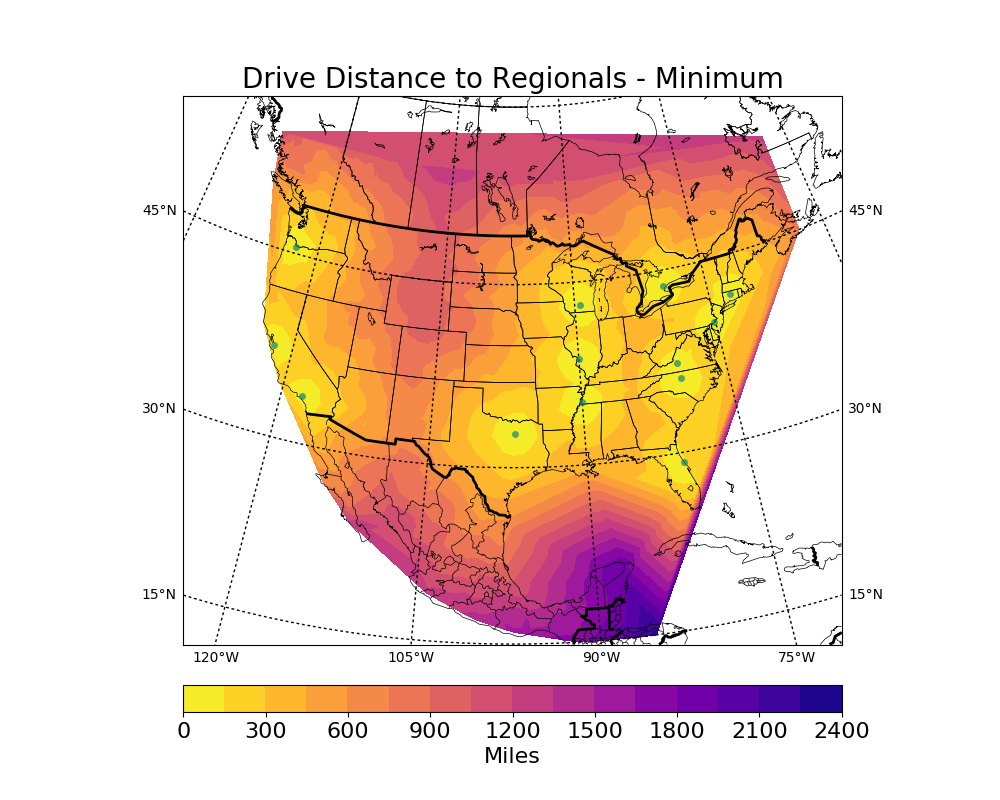
\includegraphics[height=.3\textheight]{../figs/Figure_3}
\end{subfigure}%
\begin{subfigure}{.5\textwidth}
  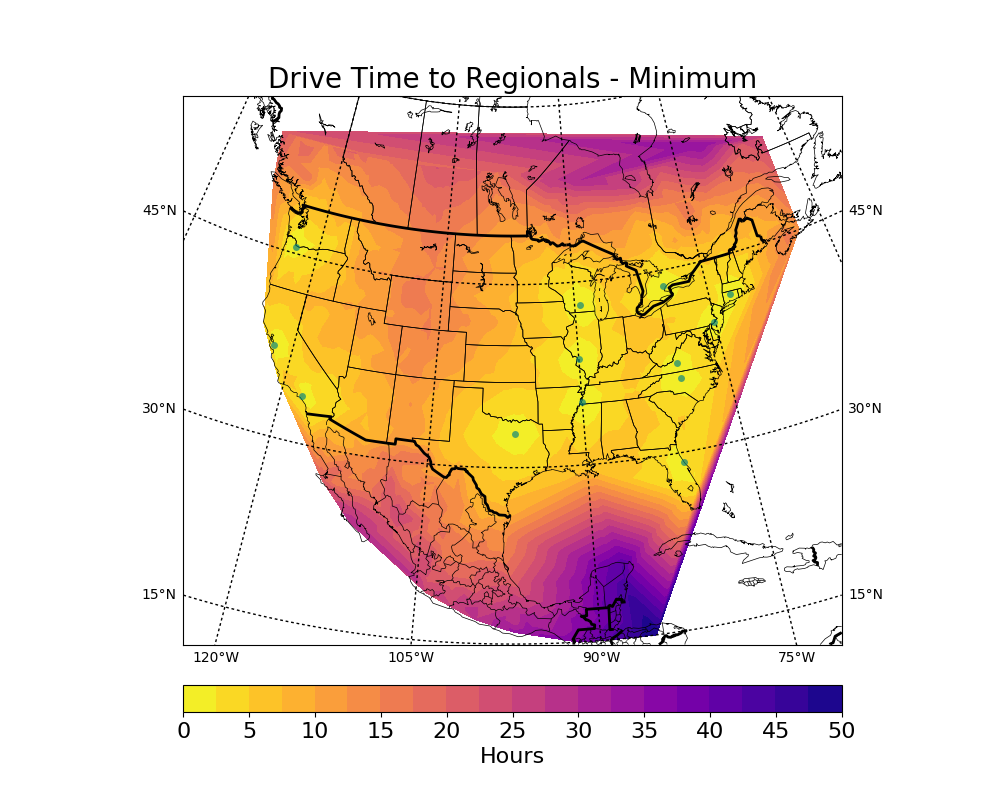
\includegraphics[height=.3\textheight]{../figs/Figure_4}
\end{subfigure}%
\newline
\begin{subfigure}{.5\textwidth}
  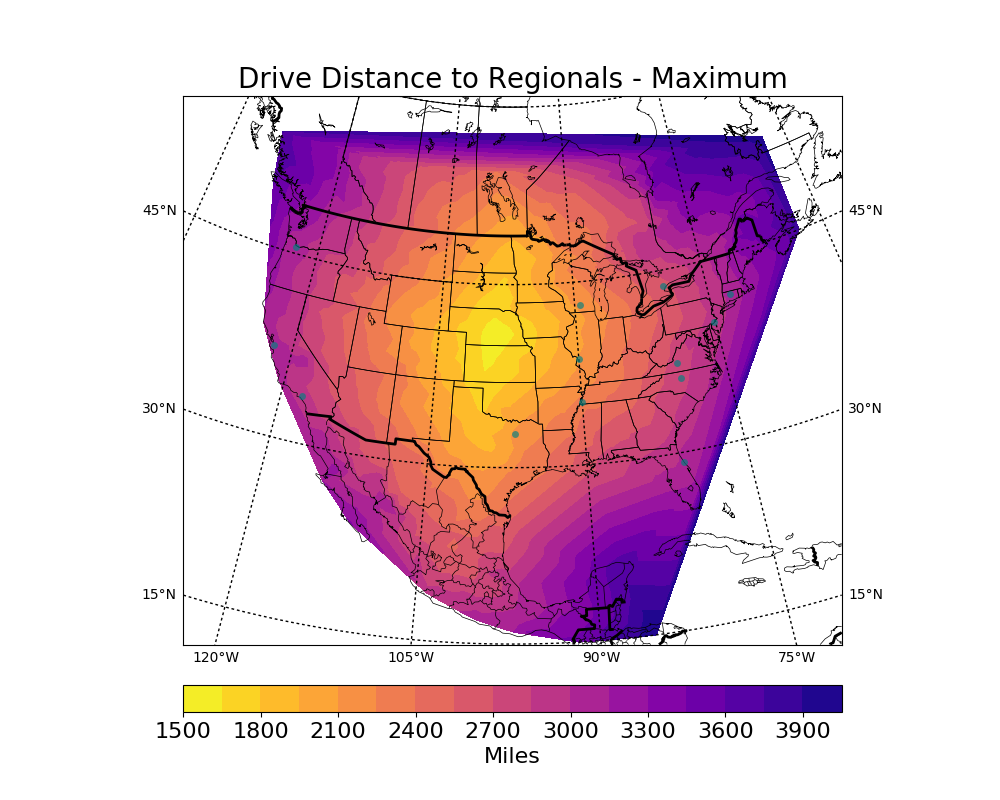
\includegraphics[height=.3\textheight]{../figs/Figure_5}
\end{subfigure}
\begin{subfigure}{.5\textwidth}
  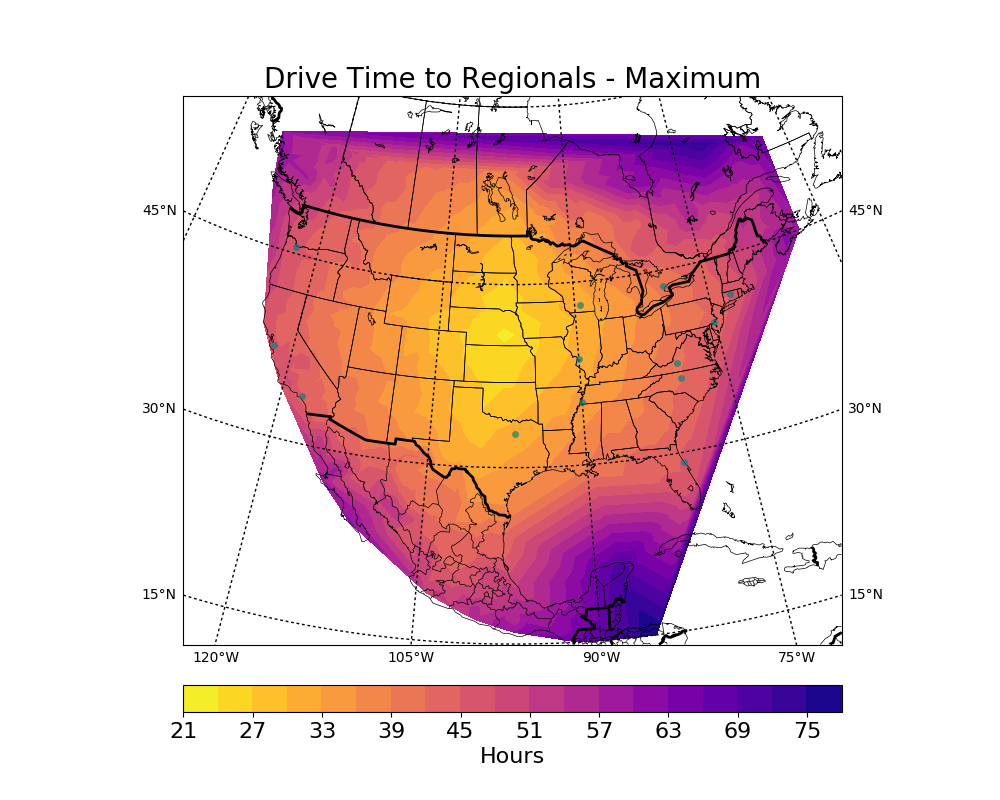
\includegraphics[height=.3\textheight]{../figs/Figure_6}
\end{subfigure}
\begin{subfigure}{.5\textwidth}
  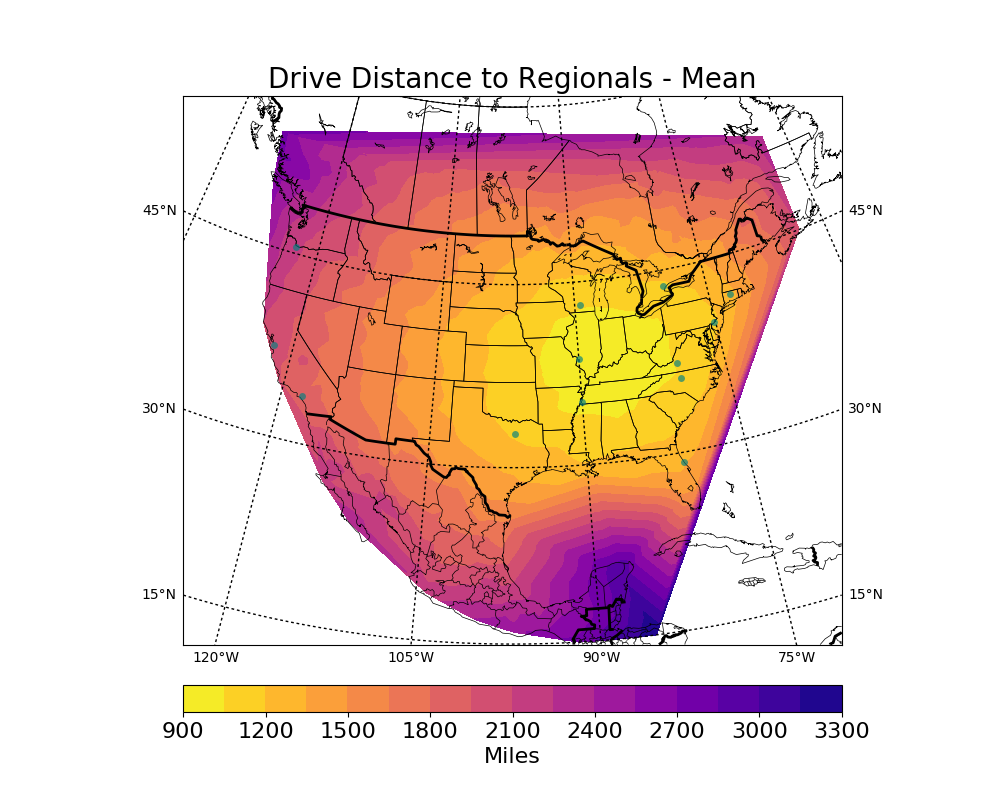
\includegraphics[height=.3\textheight]{../figs/Figure_7}
\end{subfigure}
\begin{subfigure}{.5\textwidth}
  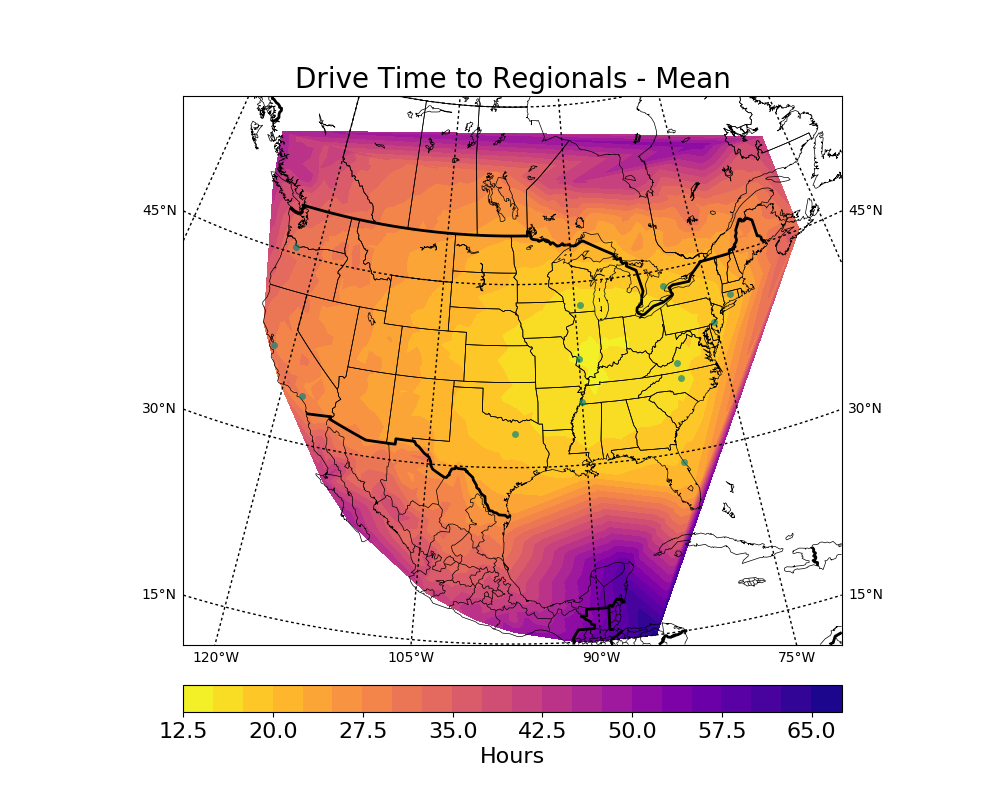
\includegraphics[height=.3\textheight]{../figs/Figure_8}
\end{subfigure}
  \caption{Plots of drive time (left) and drive distance (right) statistics to the Regional events.}
\end{figure*}

\begin{figure*}
\begin{subfigure}{.5\textwidth}
  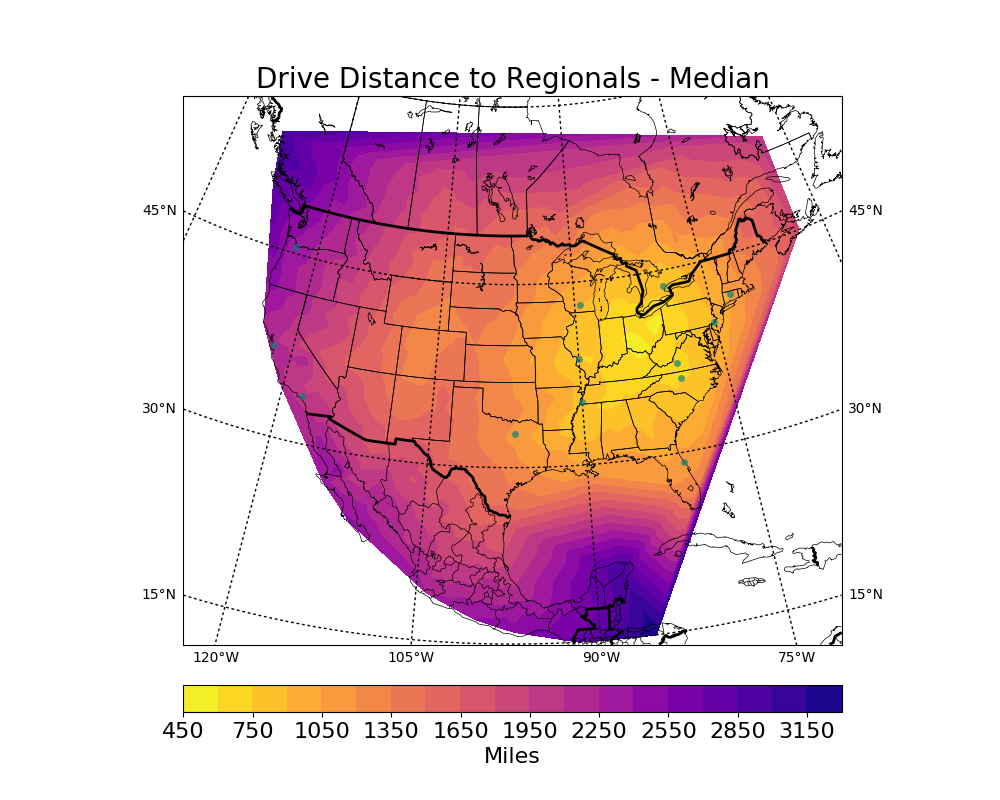
\includegraphics[height=.3\textheight]{../figs/Figure_9}
\end{subfigure}
\begin{subfigure}{.5\textwidth}
  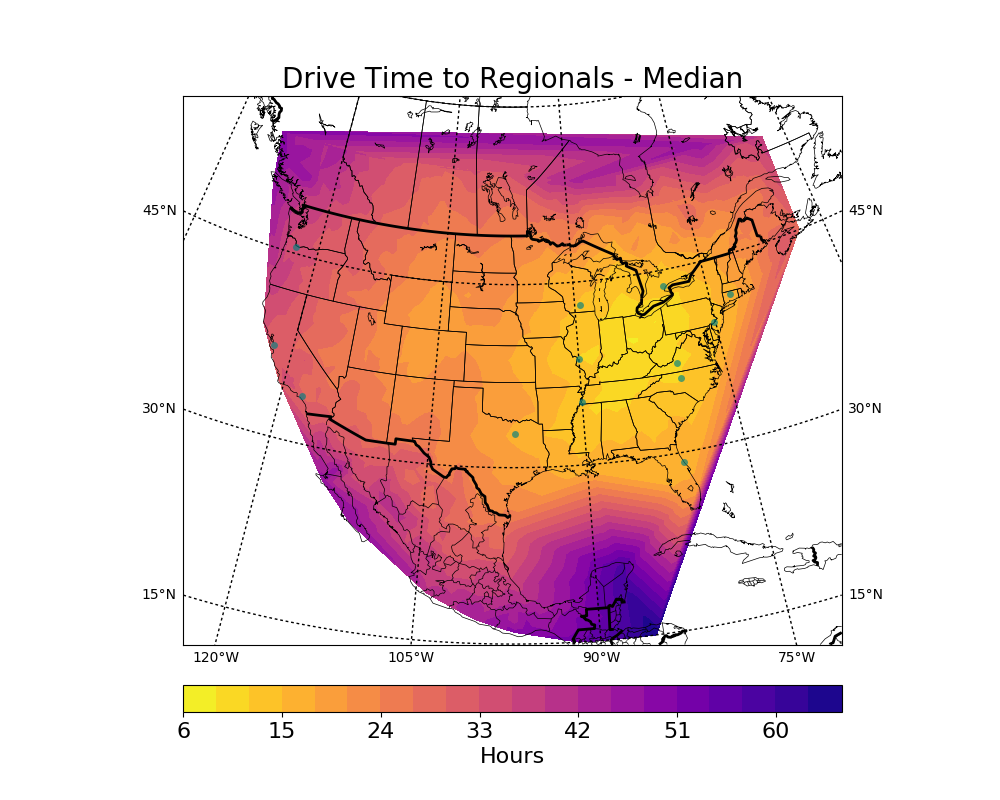
\includegraphics[height=.3\textheight]{../figs/Figure_10}
\end{subfigure}
\begin{subfigure}{.5\textwidth}
  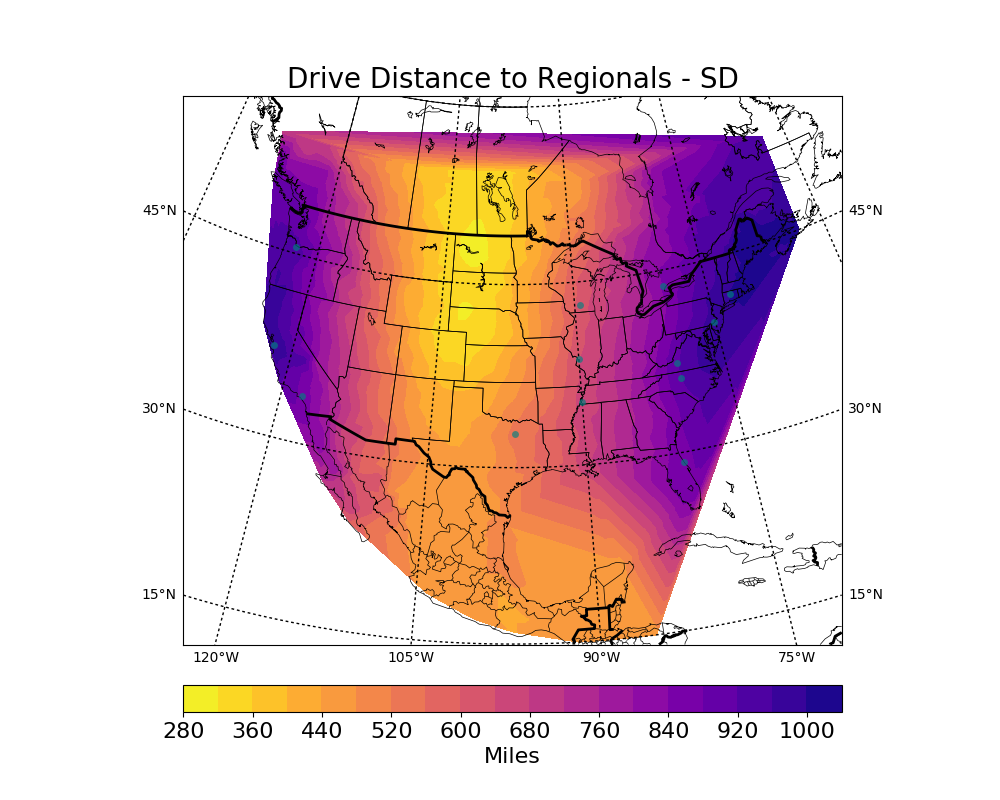
\includegraphics[height=.3\textheight]{../figs/Figure_11}
\end{subfigure}
\begin{subfigure}{.5\textwidth}
  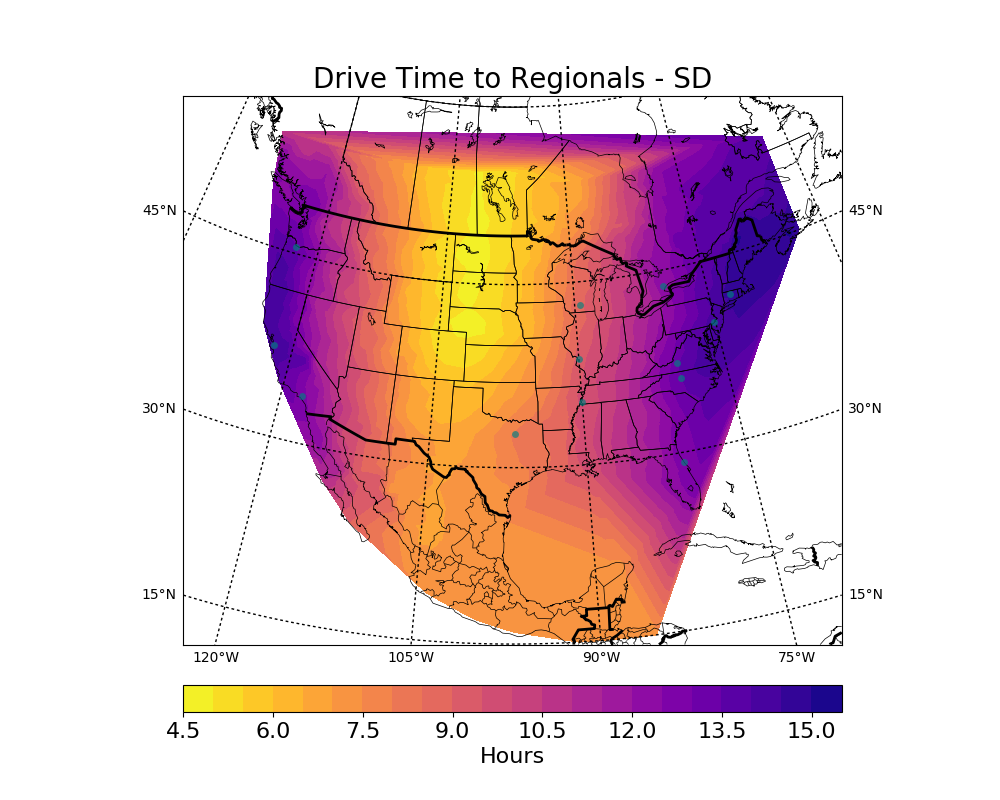
\includegraphics[height=.3\textheight]{../figs/Figure_12}
\end{subfigure}
  \caption{(cont.) Plots of drive time (left) and drive distance (right) statistics to the Regional events.}
\label{fig:fig}
\end{figure*}

Looking at the minimum drive times and distances we notice a trend running North-South through MT-WY-CO-NM and into Mexico. This represents the area of the US that is most affected by the location of the Regionals. MT and WY have about a 20 hour drive to their closest Regional, CO has roughly a 14 hour drive. If you're in Canada or a country south of the US border, you either live lose to the boarder or you have a long drive of 15-50 hours. 

The maximum driving distance provides an interesting perspective because it gives us an upper bound on travel time. Each color gaurentees that all Regional events are under a certain driving distance. It's also a measure of the central location of where Regionals are located. In this case, it's in the middle of NE and gaurentees that all Regionals are under a 21 hour drive. If you're looking to hit all of Regionals, and travel cost is a concern, you might consider moving the NE. Obviously, the edges of the map have the highest max travel time, as there will always be a Regional on the other coast. 

The means and medians show us where the Regionals are clustered and where people should live if they want to drive to a fair number of Regionals, but stay more local. The mean shows us that the area around Collinsville, IL has the lowest mean travel time at about 12.5 hours. If we recall the September report, we know that the mean is sensitive to outliers (one being a nearly 0 hour tavel time to Collinsville Regionals), and if we want to disregard those we should use the median instead. The median is centered on the great state of OH, sporting a healthy 6 hour median travel time. The problem with the median in this case is that it ignores small and large outliers, but if a Regional was in a player's hometown, state, city, or general geographical area, they are more likely to attend rather than not. What really should be done in this case is to ignore large outliers, but keep the small by some kind of weighted average measure. However we're saving that for future work.

The standard deviation is also an interesting measure. It basical tells us how consistent the drive times are throughout the Regionals circuit. We notice that the mid-US actually benefits from this statistic. Any one Regional they choose is likely to be the same distance away as any other Regional. We know that the distance is going to be high from the Min and Max maps, but it removes distance as a factor when considering which Regional to attend. The coasts have a high standard deviation, which means they're more likely to consider distance when choosing an event to attend, and that they're more likely to attend Regionals that are closer to where they live. 

\section*{Special Section: Worlds 2018}

Where do World's players come from and does the circuit reflect that? This is an important question to ask when analyzing the Regionals circuit. The way that the Regionals circuit is laid out spatially suggests that there are regions which are more likely to favor players trying to make Worlds while making it hard for others without extensive travel. Top players have, in the past, bragged about earning all of their CP from Regional events and never having to attend their local events. Politics of that aside, if these players come from a region with a high density of Regionals, it suggests the circuit enabled or helped their Worlds invite in some way. If the players come from a region that is sparse in Regionals (i.e. Montana), it suggests that the circuit is more balanced. From the maps in the previous section, we already know that the circuit isn't fair or balanced spatially, but let's go through the data regardless.

This data was collected by finding the top Masters CP earners in the US during the 2018 circuit on TPCi's Organized Play website and cross referencing names with public Twitter accounts and VGCStats tournament results to get a rough sketch of where the players who received Worlds invites play. It is by no means a complete list, and the locations are inexact, but still useful. 

\section*{Discussion and Conclusion}



In closing we'd like to thank the \href{vgcstats.com}{VGC Stats Project} for hosting this and other great articles. The data is freely avaliable to download from the \href{https://docs.google.com/spreadsheets/d/1ma2g3MTRTx3fUCun9awvshfAFoD9gRbB7rpf7qXve-k/edit?usp=sharing}{2018-2019 US VG Event Info Sheet}. The source code to generate this report is avaliable on \href{https://github.com/ckohnke/pkmheatmap}{Github}. The compiled monthly reports can be found in PDF form on Github, or at this Google Drive \href{https://drive.google.com/drive/folders/1hMER-3G8YYeeNijA68x8WsmD1cQDyu9X?usp=sharing}{link}. As always, if you have any suggestions, want to lend a hand, or just want to tell us we're doing a great job, feel free to reach out on Twitter \href{https://twitter.com/clearcreekVG}{@clearcreekVG} (Colton) or \href{https://twitter.com/PokenomicsDMV}{@PokenomicsDMV} (Kyle), or any other means you have of contacting us. 

\end{document}
